\documentclass[12pt, man, a4paper, floatsintext]{apa7}
    
\usepackage[utf8]{inputenc}
\usepackage{csquotes}
\usepackage{amsmath, amssymb}

\usepackage{graphicx}
\graphicspath{{../figures/}}

\usepackage[style=apa, sortcites=true, backend=biber]{biblatex}
\addbibresource{references.bib}


\title{A Machine Learning Approach to Equity Bubble Detection and Market Crash Prediction}
\shorttitle{Machine Learning to Bubble Detection}
\author{Hongkai Yu}
\affiliation{{Vancouver School of Economics, University of British Columbia
          \\ ECON 490
          \\ Dr. Jonathan Graves
          \\ April 23, 2021}}

\abstract{
In this research, I aim to detect equity bubbles and predict financial crashes in the S\&P 500 index. I implement machine learning models with special consideration to the imbalanced data problem. The imbalanced data problem refers to the fact that there are far more non-bubbles than bubbles in the training data. The problem makes the model undesirably fits too much on non-bubbles. Features of the models are selected based on economic theories and market fundamentals. I find that the Random Forests model with Cross-Validation-tuned decision threshold performs the best, with a 93.0\% balance accuracy rate. The balanced accuracy is the average of sensitivity (100\%) and specificity (86\%). The Recurrent Neural Networks with Bidirectional Long-term Short Memory and focal loss function gives unsatisfactory results, possibly due to the modest data size. Features with the highest predictive power are market fundamental indicators, long-term market returns, and the psychology factor. Short-term market returns and macroeconomic indicators are less important for the prediction of market crashes. The model in this research is limited to predicting long-term (more than 3 months) and extreme market downturns. }

\keywords{
Asset Bubbles, Market Crashes, Machine Learning, Deep Learning, Random Forests, Recurrent Neural Networks
}


\begin{document}

    \linespread{1} % for tables

    \maketitle

    \section{Introduction}
    
Bubbles and market crashes are important themes of financial markets. Asset bubbles describe the situation where asset prices significantly deviate from their fundamental values. Notable historical bubble includes the Dutch tulip mania in 1637, the dot-com bubble in the 1990s, and the US housing bubble in 2000s. Investors who are unaware of the potential risks of bubbles realize huge losses when bubbles burst and the market crashes. Some people believe the market crash in 1982 wiped out the cumulative profits of the history of American banking history \parencite{blackswan}.

More recently, despite the general economic downturn caused by the COVID-19 pandemic, stock markets are performing exceedingly well. The S\&P 500 index was up by 18.23\%, while the tech-heavy NASDAQ gained 43.6\% in 2020. With the historical lesson of bubbles, we may wonder if we are experiencing one right now.

Given the catastrophic consequences caused by bubbles, it would be meaningful if we can identify bubbles and predict potential crashes. An accurate bubble detection tool may serve as an early warning system for policymakers or a risk management tool for investors. Building such a bubble detection tool is the primary motivation of this research. While bubbles and market crashes are broad phenomena, in this paper, I focus on bubble detection in the stock markets. Specifically, the scope of the research is limited to bubble detection in the S\&P 500 market index. The main research goal is to come up with a method that can reliably detect equity bubbles and forecast market crashes in the S\&P 500 index. 

If we can realize the main research goal, we can answer certain further questions. Assuming that the prediction method is transparent enough, we can identify important factors that are the most important for prediction. On the technical side, we can gain insights into the selecting empirical methods that work the best for equity bubble detection problems. Also, we can predict if we are in an equity bubble right now using our proposed prediction method. 

There is much previous research done in the field of bubble detection and market crash prediction. Some researchers, based on economic theories such as rational choices and fundamental value as discounted dividends, came up with statistical tests like variance bound test for bubble detection \parencite{shiller1980}. More recently, researchers have applied machine learning methods, which are powerful prediction tools for detecting complex patterns, to the study of predicting market crashes \parencite{Chat2018}. However, as we will see in the literature review section, previous studies are limited in two ways. First, the theory-based studies are highly reliant on their theoretical assumptions and suffer from problems such as joint hypothesis testing. Second, model-free machine learning studies typically do not include enough input variables. They only include short-term trading variables and have unsatisfactory prediction power. 

I attempt to solve these limitations in this paper. To avoid the theory reliance problem, I adopted the definition of bubble purely from observable data. As readers may have noticed, I have used the term “bubble” interchangeably with potential market crashes. That is precisely my definition of bubbles. While it may not be suitable for theoretical debates, e.g., “do bubbles exist”, it captures the practical side of the concept of bubbles for practitioners like policymakers and investors. With this definition, the bubble detection problem is transformed into a supervised machine learning classification problem, where we try to predict the output, the bubble, given the input variables. One of the distinguishing features of this research is that I include more input variables than many previous studies to boost the prediction power of models. I select variables that are suggested by economic theories as input variables for bubble detection, including macroeconomic data, long-term trading trends, and market fundamental indicators. It is worth noting that the validity of my research would not be dependent on the correctness of theories, because they are merely serving as feature-selection tools.

I implemented three machine learning models as candidates for the best classifiers: logistic regression (logit), Random Forests (RF), and Recurrent Neural Networks with Bidirectional Long Term Short Memory (RNN-BiLSTM). Logistic regression is easy to implement and can be well interpreted. Yet compared to the other two methods, it is limited that it restricts the function form to linearity after the logistic transformation. The RF model is good at detecting non-linear patterns, and it seems promising based on a previous study. RNN-BiLSTM has been found to have superior results with financial time series data compared to traditional methods. Besides, it is used in similar studies and has good performance. 

One unique challenge of the modelling is that the dataset is imbalanced, meaning that there are far more non-bubble instances than bubbles. I have adopted special techniques to mitigate this problem, for example, re-sampling for re-weighting, changing decision thresholds, and using asymmetric loss functions. I also use balanced accuracy, which is the average of specificity and sensitivity, as my model evaluation metric.

The results of the research are satisfactory. I have met the main research goal of finding a high-performing model. My best performing model, the RF with CV-tuned decision thresholds (RF-CV), achieves a balanced accuracy of 93.0\%. It can reliably detect equity bubbles and predict market crashes. For variable importance inference, I find that long-term market returns and market fundamental indicators are the most important factors, whereas short-term market returns and macroeconomic data have weak predictive power. On the technical question of the efficiencies of empirical methods, the research confirms that machine learning is an effective way of detect equity bubbles and predict market crashes. Among the machine learning models, RF models have the best performance, followed by logit models. This is expected since RF models can capture the non-linear relationships that cannot be detected by logit models. RNN models have unsatisfactory results, possibly due to the insufficient size of training data. This implies that the deep learning techniques should be used with caution since they do not always guarantee high performance. Finally, the best performing model, the RF-CV, shows that we are likely in a stock bubble as of April 2021, and market crashes are likely in the next six months.

The research has two main contributions. First, I use a new methodology that takes advantage of both the power of machine learning algorithms and the feature-selection insights from economics theories. This methodology avoids the theory dependence problem such as the joint hypothesis problem and can boost the model performance by including more features. Second, I build a high-performing predictor (RF-CV) for detecting equity bubbles and predicting market crashes. To the best of my knowledge, it is the highest-performing machine learning model for predicting market crashes. I believe this can be used as a useful tool for financial market practitioners.


The rest of the paper is organized as follows. The background section provides a literature review of previous research and my motivation for this research. The data section lists all the input variables, their theoretical justification of relevance, and my definition of the output variable, the bubble. The model section introduces the machine learning models that I selected and the reasons for choosing them. The model section also introduces the methods to mitigate the imbalanced data set problem. The result section presents the model performance and the inference of variable importance. The discussion section provides model diagnosis, conducts a robustness analysis, and discusses the limitation of the research. Finally, the conclusion section summarizes the key findings and the contributions of this research.

    \section{Background}

Much previous research has been done in the study of bubble detection and financial crisis prediction. However, I find previous research is limited in two ways: too many theoretical assumptions and not enough feature inclusion. In this section, I will give a literature review of the previous research and explain my motivation for this research.

There is plenty of theoretical research on asset bubbles. At the foundation level, it is still debated whether bubbles exist. Eugene Fama, the proposer of the Efficient Market Hypothesis (EMH), is generally skeptical of the notion of the bubble \parencite{fama2014}. He argues that people should not use the word \textquote{bubble} without careful definition and empirical validation. For those who believe in the existence of bubbles, their views on the cause of bubbles diverge. As described by \textcite{Wckl2019Survey}, bubble models can be categorized into rational bubble models and behavioural bubble models, i.e., irrational bubble models. 

The family of rational bubble models relies on the rational decision-making assumptions of the agents. They typically explain bubbles by asymmetrical information and the herding behaviours of investors. For example, \textcite{allen1993} argues that if the beliefs of participants are private, an asset bubble is possible when all participants rationally believe they can sell the stock to a new buyer \textquote{before its true value is publicly revealed.} On the other hand, behavioural bubble models do not presume the rationality of agents. Irrational behaviours are central to the behavioural bubble models. For instance, it has been found that people are generally biased as they rely on representativeness for the decision-making \parencite{TVERSKY1973207}. In the financial markets, this effect can cause people to overact on market news and lead to biased pricing of the asset \parencite{psychology}. 

The interest in bubbles is not limited to theoretical research. On the empirical side, the phenomenon of bubbles is of great importance to policymakers and investors since an expected bubble could lead to huge losses. Researchers have tried various methods to accurately detect bubbles.

Some researchers believe that the high volatility of the stock price signals underlying bubbles. Since the fundamental value of the stock is unlikely to change rapidly, they argue, the high volatility must be due to irrational, speculative behaviours. Following this line of thought, \textcite{shiller1980} proposes the variance bound test for bubble detection. If the variance of the stock is higher than a given bound, we can reject the null hypothesis of no bubble. Later research aims to test whether the time series variable of the bubble is stationary. Similar to the reasonings for volatility, researchers hold that the variables related to the asset should be stationary if there is no bubble. \textcite{craine1993} employs the Augmented Dicky-Fuller (ADF) test to check whether the price-dividend ratio is stationary. He argues that if the ADF test rejects the null hypothesis of stationary, a rational bubble is likely.

However, these econometric empirical tests are not without criticism. A survey conducted by \textcite{Gur2008} finds that the conclusion of the econometric tests of bubbles is uncertain. He finds that models that fit data equally well can have different conclusions as to whether a bubble exists. Even if the results of the econometric test are conclusive, he argues, it is not sufficient to demonstrate the existence of bubbles. It could be that the assumptions of the models are questionable. As noted by \textcite{Wckl2019Survey}, many the econometric tests suffer from the joint hypothesis testing problem: since the test depends on models, the test is simultaneously testing against the assumption of no bubble and the validity of the model assumptions. It could be the failure of any other model assumptions that lead to the rejection of the null hypothesis. Also, \textcite{evans1991} finds that the stationary tests for the bubble are flawed in that they cannot detect \textquote{an important class of rational bubbles.}

Contrary to the econometric tests approach of bubble detection, some researchers choose to directly model the practical consequences of the bubble: market crashes. While econometric tests depend on their model assumptions, which are often unobservable and untestable, market crashes are directly observable. \textcite{jacobsson2009} proposes a method called Log-Periodic Power Law to detect speculative bubbles. More recently, researchers use advanced machine learning methods to study the pattern of market crashes. Machine learning methods are powerful in capturing complex patterns in the data. \textcite{Chat2018} uses models including Support Vector Machines, Random Forests, and Deep Neural Networks for predicting crisis on the 20-day horizon and 1-day horizon. \textcite{Bash2020} and \textcite{Moser} uses Recurrent Neural Networks (RNNs) with Long short-term memory (LSTM).

However, these studies typically include few types of features. \textcite{Bash2020} and \textcite{Moser} use almost exclusively daily prices of the stocks or market indexes. The features included in \textcite{Chat2018} are primarily stock variables and bond market data. 

Given the academic context, I aim to solve the limitations of the previous research. In light of the model-reliance problem of econometric tests, I choose the model-free machine learning approach for this research. On the other hand, I improve upon previous machine learning studies for market crashes by including more variables as feature. The features are suggested by economic theories as relevant to the financial market performance. An introduction of the data is presented in the next section.

    \section{Data}

In this section, I will give an overview of the data used in this research. First, I will introduce the input variables, a.k.a., features, and my reasons for selecting them. The features include macroeconomic data, market return trends, and market fundamental indicators. Then, I will explain my definitions of equity bubbles and financial crashes. The range of the data is from January 1960 to December 2020 in the US. Unless otherwise specified, the frequency of the variable is monthly. The raw data are retrieved from Federal Reserve Economic Data (FRED) and \emph{multpl.com}.

\subsection{Input variable}

\paragraph{GDP growth rate} The real Gross Domestic Product growth rate measures the productivity growth of a nation. It is one of the most important macroeconomic metrics. Given its importance, sophisticated machine learning models might gain insights from the growth pattern for bubble detection. The frequency of the GDP data is quarterly rather than monthly. To make the data frequency consistent, I replicate the quarterly GDP growth rate to all the corresponding months.

\paragraph{Inflation} The growth rate of the Consumer Price Index measures the price inflation in a nation. Similar to the GDP growth rate, it is one of the most important macroeconomic indicators. In the context of financial markets, previous research finds that there is an inverse relationship between inflation and lower share prices \parencite{inflation}. It might be the case that a high level of inflation is associated with a higher possibility of market crashes.

\paragraph{T-bill yield} The 10-year Treasury constant maturity rate is a key benchmark in the debt market. It captures the long-term expected yield of a risk-free investment. From the perspective of an investor, the debt investment and the equity investment are substitutions. It has been found that bond returns tend to be higher than stock returns when the market uncertainty increases \parencite{bond}. There is reason to believe that inflation could help detect equity bubbles. 

\paragraph{S\&P 500 returns} The Standard \& Poor is one of the most widely used stock market indexes. It measures the stock returns of the largest 500 companies listed in the US. As discussed in the following subsection, the output variables — equity bubbles and market crashes are constructed from S\&P 500 returns. As a common practice in time-series forecasting, it is natural to use historical returns to forecast future data. To include the price trends in different periods, I include 1-, 3-, 6-, 12-, 60-month returns of S\&P 500 as features.

\paragraph{Consumer confidence} As noted by \textcite{psychology}, the psychological factors of investors have a significant influence on investment decisions. I use the data of consumer opinion surveys as a proxy for the public sentiment of the general business environment. While the capital market sentiment does not always align with consumer confidence, this is the most easily accessible data. Also, unlike other newly invented stock market sentiment indexes,  the consumer confidence data is complete between 1960 and 2020.

\paragraph{Shiller P/E ratio} Invented by \textcite{shiller2015IE}, the Shiller P/E is also known as the cyclically adjusted price-to-earnings ratio. It measures stock prices as a ratio to the average inflation-adjusted earnings \parencite{shillerPE}. If the Shiller P/E ratio is too high, it suggests that the stock prices could be overvalued based on the corporate earnings. 

\paragraph{Market capitalization-to-GDP ratio} Warren Buffet believes that \textquote{the market value of all publicly traded securities as a percentage of the country's business} is a useful metric for investment decisions \parencite{buffett}. Given the investment success of Warren Buffet, the effectiveness of this metric seems worthwhile to explore. Since collecting data for all publicly traded securities is cumbersome, I calculate the ratio between the S\&P 500 index and the nominal GDP as a proxy. Similar to the real GDP growth rate, the frequency of the nominal GDP is quarterly. I replicate the GDP data to match the monthly frequency.

Table~\ref{tab:features} presents a summary of input variables. \emph{Min} is the minimum value of the variable; $q_1$ is first quantile of the variable; $\tilde{x}$ is the median value of the variable; $q_3$ is the third quantile of the variable; \emph{Max} is the Maximum value of the variable; $\bar{x}$ is the mean value of the variable; $s$ is the sample standard deviation of the variable.

% latex table generated in R 4.0.3 by xtable 1.8-4 package
% Wed Apr 21 23:19:25 2021
\begin{table}[ht]
\centering
\begingroup\normalsize
\begin{tabular}{lrrrrrrr}
 \textbf{Variable} & \textbf{Min} & $\mathbf{q_1}$ & $\mathbf{\widetilde{x}}$ & $\mathbf{q_3}$ & \textbf{Max} & $\mathbf{\bar{x}}$ & $\mathbf{s}$ \\ 
  \hline
Annualized GDP Growth Rate (\%) & -31.4 &  1.4 &   3.0 &   4.7 &  33.4 &   3.0 &  4.5 \\ 
  Annualized Inflation (\%) & -19.3 &  1.5 &   3.2 &   5.4 &  24.0 &   3.7 &  3.9 \\ 
  10-year T-bill yield (\%) &   0.6 &  3.9 &   5.7 &   7.7 &  15.3 &   6.0 &  2.9 \\ 
  Shiller P/E Ratio &   6.6 & 15.0 &  20.5 &  25.7 &  44.2 &  20.6 &  8.0 \\ 
  Consumer Confidence Index &  95.7 & 98.9 & 100.5 & 101.1 & 103.1 & 100.0 &  1.6 \\ 
  Market Capitalization-to-GDP Ratio &   0.0 &  0.1 &   0.1 &   0.1 &   0.2 &   0.1 &  0.0 \\ 
  1-Month S\&P 500 Return (\%) & -20.4 & -1.2 &   1.0 &   2.8 &  12.0 &   0.6 &  3.6 \\ 
  3-Month S\&P 500 Return (\%) & -31.1 & -1.7 &   2.4 &   6.2 &  25.9 &   2.0 &  7.0 \\ 
  6-Month S\&P 500 Return (\%) & -37.8 & -2.4 &   4.5 &   9.9 &  38.0 &   4.0 & 10.6 \\ 
  12-Month S\&P 500 Return (\%) & -42.5 & -0.8 &   9.7 &  18.3 &  52.7 &   8.0 & 15.3 \\ 
  60-Month S\&P 500 Return (\%) & -32.6 &  9.4 &  45.4 &  70.4 & 213.9 &  46.1 & 46.5 \\ 
  \end{tabular}
\endgroup
\caption{Summary of features} 
\label{tab:features}
\end{table}


An interpretation of the median data in the table is the following: the real GDP growth rate of the current quarter is 3.0\% annually; the inflation rate is 3.2\% annually; the 10-year Treasury Bond yield is 5.7\% annually; the Shiller P/E ratio of the month is calculated to be 20.5; the consumer confidence is 100.5, higher than the baseline value of 100; the market capitalization-to-GDP ratio, measured by the ratio between the S\&P 500 index and the nominal GDP in the current quarter, is 0.1; the S\&P 500 returns in the past 1, 3, 6, 12, and 60 months are 1\%, 2.4\%, 4.5\%, 9.7\%, and 45.4\% respectively. 

\subsection{Output variable}

I follow the definition of \textcite{Chat2018} and define a market crash as an extreme market downturn. An extreme market downturn is a one percentile market return. Given this definition, I define the bubble as a pre-stage of market crashes. The bubble is a binary variable: at a given month, it can take the value 1, which denotes that there is a bubble, or take the value 0, which denotes that there is no bubble. As an operational definition, the bubble variable takes the value 1 if and only if: 1) there will be a market crash in the next six months; 2) the current period does not see a market crash. 

The benefit of this bubble definition is that it is entirely based on observable data. It does not involve a theoretical definition of the fundamental value of the stock nor prescribe the behaviours of investors. As discussed in the background section, these theoretical discussions could make the model depend on the assumptions of theories. They would limit the power of bubble detection models. Of course, the bubble definition in this research is not suited for a theoretical debate of bubbles. It only aims to offer empirical value for financial market practitioners.

In the above definitions, \textquote{one percentile} and \textquote{six-month} may seem to be arbitrary choices. Indeed, there is no obvious reason why we should not use \textquote{two percentile} and \textquote{five months} for the definitions. In the discussion section, I will alter the percentile and period length for robustness analysis of the model.

Figure~\ref{fig:bubble_def} shows the bubble categories through time. From the graph, we see that our bubble definition correctly identifies most pre-stages of historical market crashes, including the dot-com crash around 2001 and the US housing market crash around 2008. This confirms that our bubble definition is in line with reality.

Table~\ref{tab:imbalance} shows the distribution of output data. We see that non-bubble cases are much more than bubble cases. This is not unexpected since bubbles are abnormal market phenomena. However, as we will see in the next section, this imbalanced nature of the output variable would create a problem for modelling. 

\begin{figure}
    \centering
    \caption{The definition of bubbles}
    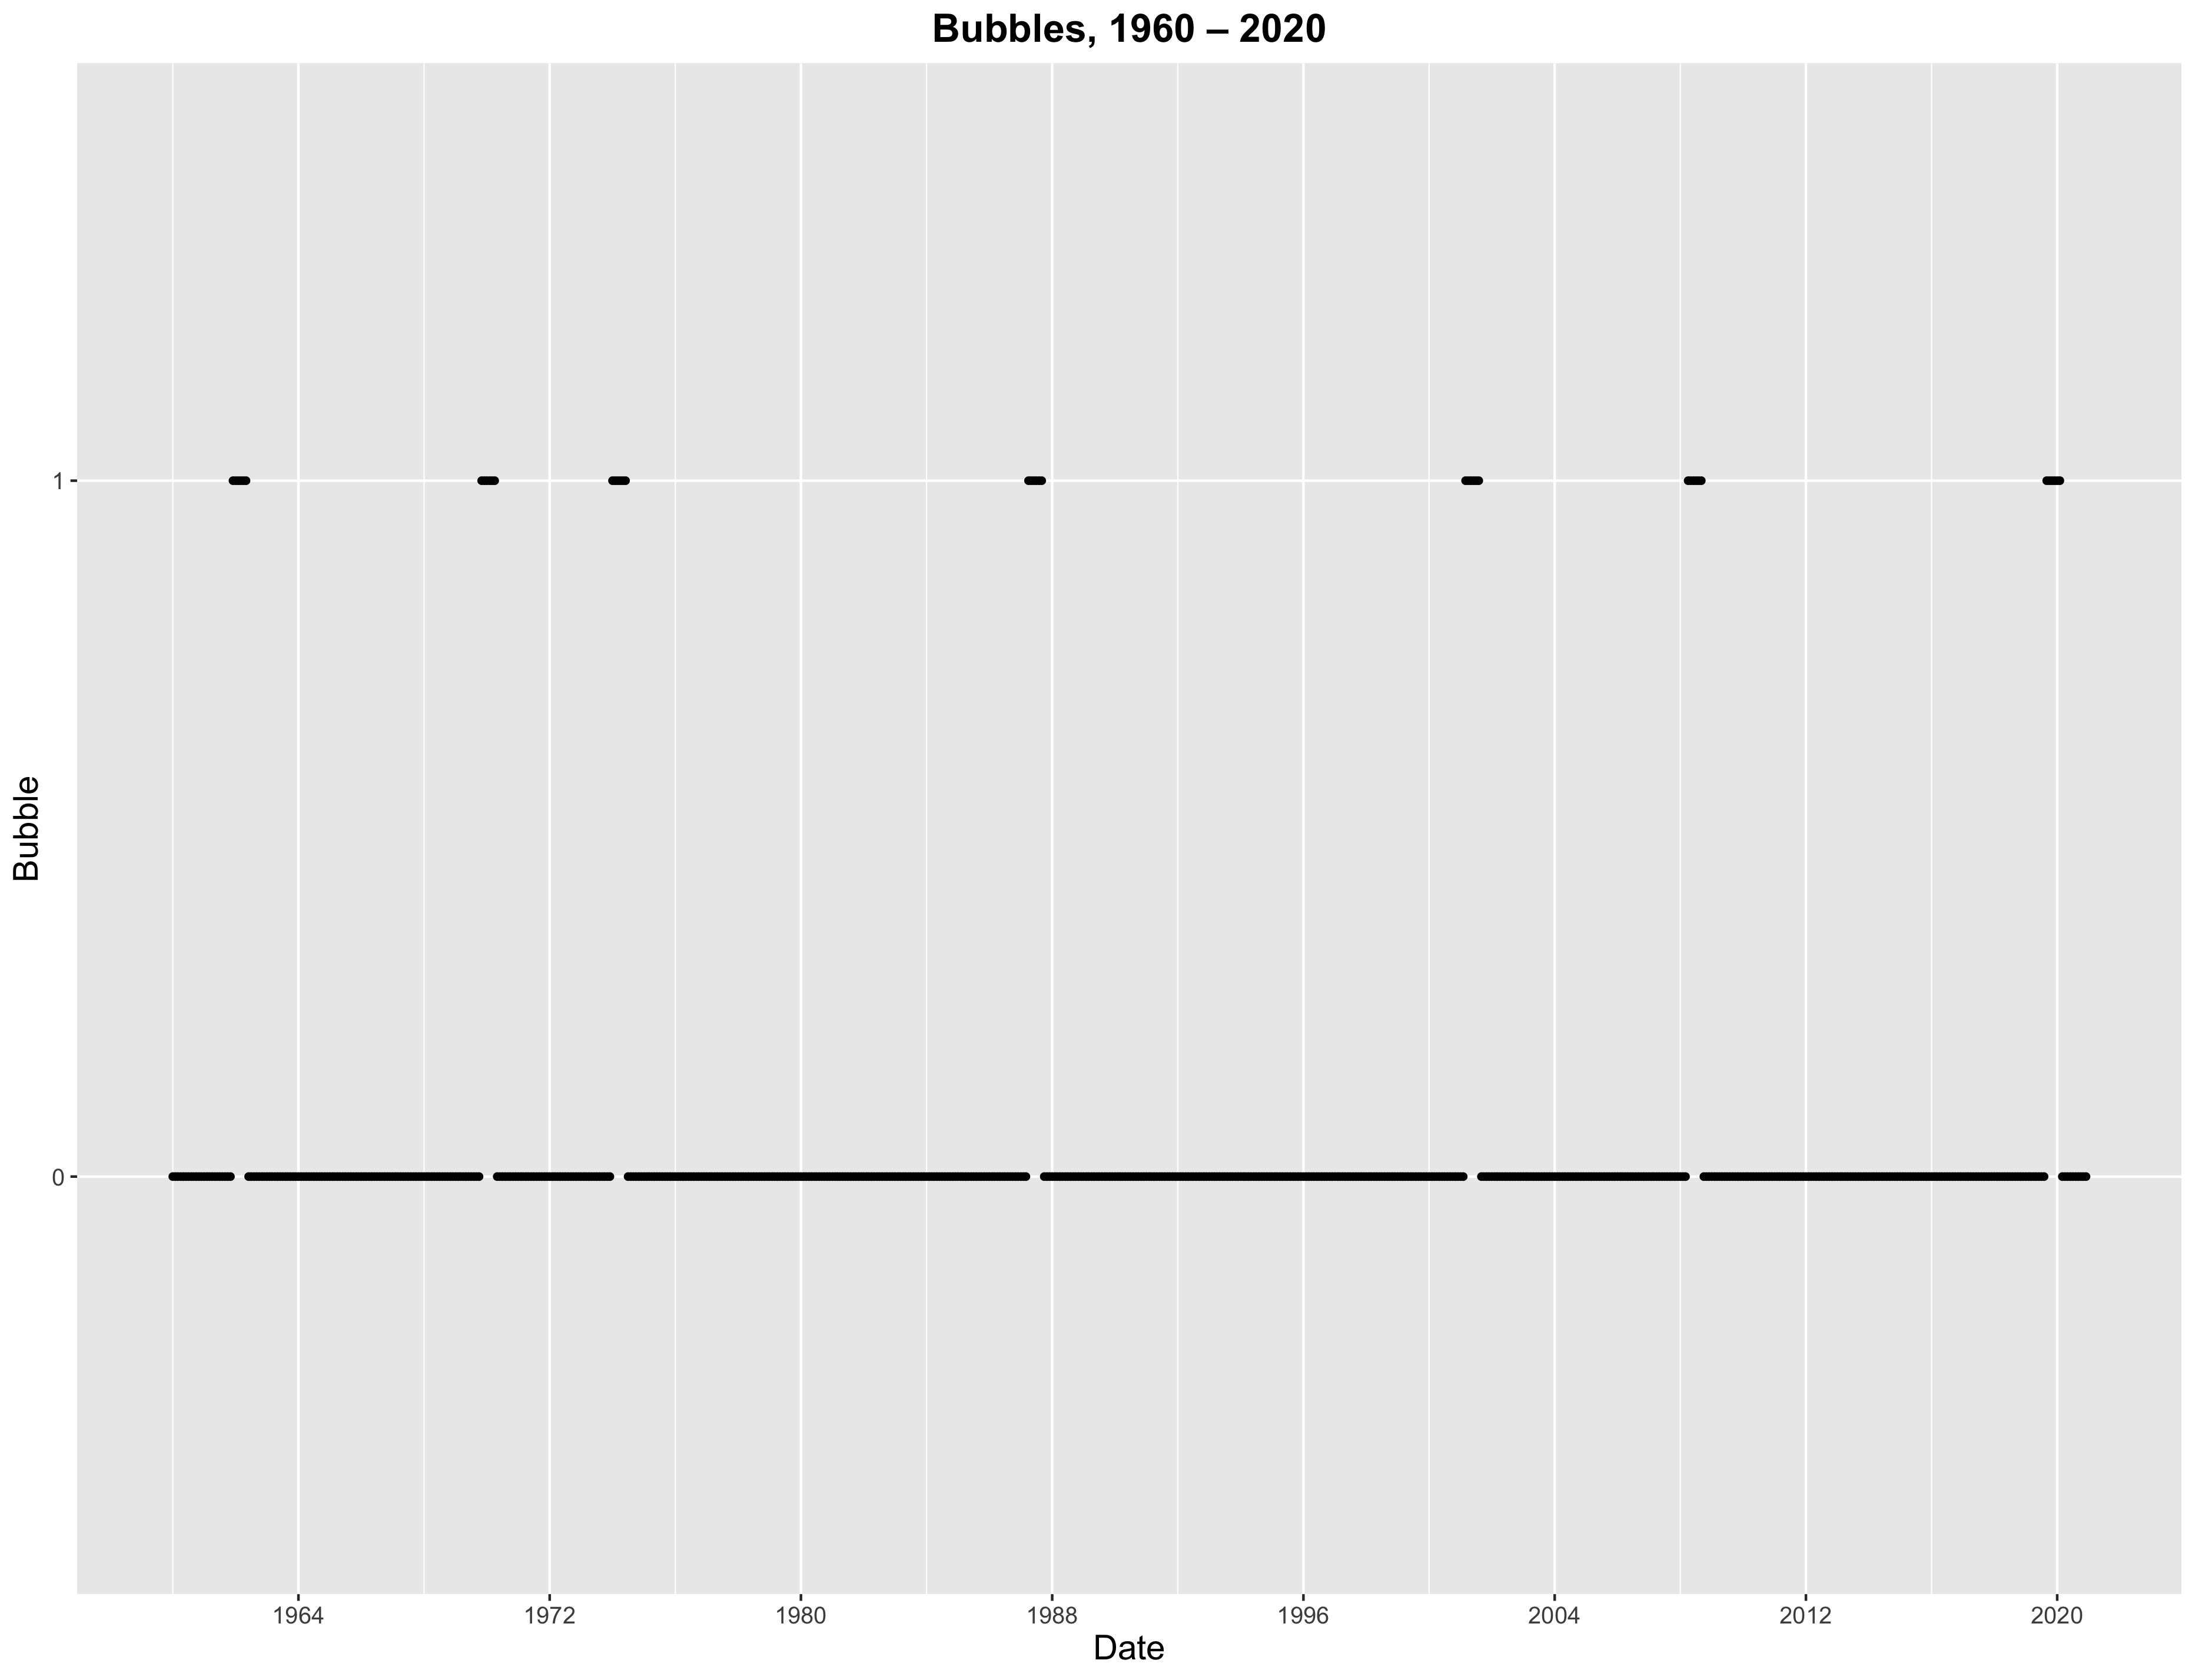
\includegraphics[width=15cm]{bubble_def.png}
    \label{fig:bubble_def}
\end{figure}

% latex table generated in R 4.0.3 by xtable 1.8-4 package
% Sun Apr 18 16:32:43 2021
\begingroup\footnotesize
\begin{longtable}{ll|rrr}
 \textbf{Variable} & \textbf{Levels} & $\mathbf{n}$ & $\mathbf{\%}$ & $\mathbf{\sum \%}$ \\ 
  \hline
bubble & 0 & 683 & 93.3 & 93.3 \\ 
   & 1 & 49 & 6.7 & 100.0 \\ 
   \hline
 & all & 732 & 100.0 &  \\ 
   \hline
\hline
\hline
\caption{Bubble distribution} 
\label{tab:imbalance}
\end{longtable}
\endgroup


Finally, as a typical practice for machine learning problems, I randomly split the full data into the training data and the testing data. The training data is 80\% of the full data, while the testing data is the remaining 20\%.

    \section{Model}

With the data set up in the previous section, the central question of the research becomes a supervised binary classification problem: we aim to predict the output variable given input variables through machine learning models. In this section, I will give an introduction to the models that I used in this research. Also, I will explain a special modelling challenge in this research — the problem of imbalanced data, and the ways to mitigate the problem.

\subsection{Model selection}

In this research, I fit three models to the data: logistic regression (logit), Random Forests (RF), and Recurrent Neural Networks (RNN).

\subsubsection{Logistic regression}

Logistic regression is one of the most widely used binary classifiers. It is easy to implement, and the interpretation of its results is straightforward. Logistic regression predicts the probability of the binary output variable through the logistic transformation. Equation~\ref{eq:logit} shows the formula of the logistic regression, where $X$ is the design matrix of the input variables and $Y$ is the output variable, the bubble. From the formula, we see that the logistic transformation of the probability of bubbles is just the log-odds of bubbles. Therefore, we can also interpret the logistic regression as modelling the log-odds of the bubble using linear models. 

\begin{equation}
    \text{logit}(P(Y)) = \log{\frac{P(Y)}{1-P(Y)}} = X \beta
    \label{eq:logit}
\end{equation}

While the logistic regression is easy to implement, it is limited in that it cannot capture the non-linear pattern in the data. The relationship between the input variables and the dependent variables (after the logistic transformation) is restricted to a linear form. However, bubbles and financial markets are complicated, and it is reasonable to assume that the true relationship is more than linearity. This is why I employ more complex models such as Random Forests and Recurrent Neural Networks to learn the non-linear pattern in the data.

\subsubsection{Random Forests}

The RF is an ensemble learning method based on decision trees. It fits many decision trees to the data through bootstrap and randomly excluding some features. Then, it aggregates the predictive results of a bag of decision trees to yield the final result. Thanks to the cursive splitting algorithm of the decision tree and the bagging method, the RF is good at detecting non-linear patterns in the data. Besides being a non-linear classifier, the main advantage of the RF is that the bagging mitigates the overfitting problem of the simple decision trees algorithm. Also, the RF is a promising method for finance research. According to a study conducted by \textcite{LinSurvey}, soft classification techniques, including ensemble learning methods, “appear to be the direction for future research” in financial crisis prediction. The nature of financial crisis studies is similar to the study of market crashes. It is reasonable to assume that the techniques which work well for financial crisis studies could also yield good results for this study. As a strong ensemble learning classifier, the RF method is a candidate for the best performing model in this research.

Besides the predictive power, the RF is also good for inference. Unlike many other advanced machine learning methods, the RF enables us to conduct variable importance analysis. Since the RF is constituted of a bag of decision trees, it can calculate the importance of a feature by comparing the decision tree performance with and without the input variable. If the inclusion of an input variable increases decision tree performance significantly, it means the input variable is important for making the prediction. This inference power of the RF is valuable for this research because one of our research questions is to identify factors that are important to prediction.

\subsubsection{Recurrent Neural Networks}

Deep learning models, or artificial neural networks with multiple hidden layers, are becoming popular in finance research. They are shown to have superior results to traditional machine learning methods. The RNN is a family of deep learning methods that are good at predicting sequential data, including time-series data. In this research, I choose a specific type of RNNs — RNNs with bidirectional long short-term memory networks (RNN-BiLSTM). The long short-term memory (LSTM) is a neural network unit that helps the model to learn from the long-term pattern in the data. The bidirectional component enables the model to detect patterns in the sequential data in two ways. Readers who are interested in knowing more about how the RNN models work can refer to \textcite{lstm} and the appendix of \textcite{Bash2020}.

In the context of forecasting financial time series, previous research has shown that RNNs with BiLSTM generally perform better than traditional time series prediction methods like ARIMA \parencite{Siam2019}. A recent asset bubbles detection study uses this method and gets satisfactory results \parencite{Bash2020}. Based on previous studies and the nature of my study, I select this method as a candidate for the best classifier. 

However, a drawback of the RNN is that the result would be hard to interpret. The behaviours of deep learning models are known to be \textquote{black box}, which means the results of the model are often inexplicable except for prediction. Unlike the RF, the model fitting process of deep neural networks does not shed light on the relative importance of input variables.

\subsection{The challenge of imbalanced data}

Apart from model selection, this research is also faced with a special challenge of imbalanced data. As shown in Table ~\ref{tab:imbalance}, the distribution of the output variable is highly imbalanced. There are way more zeros (“non-bubble”) than ones (“bubble”). This imbalanced distribution is expected since bubbles and market crashes are rare, yet it could cause trouble for the modelling. 

The default behaviour of a typical machine learning fitting algorithm is to minimize misclassification cases in all training data. Since the non-bubble case represents the over-majority of the data, without any special treatments, the model fitters are expected to focus more on the non-bubble cases than the bubble cases. This behaviour is undesirable because the research is interested in predicting bubbles. As an extreme case, even a naïve classifier that predicts zero in all cases would have a high accuracy rate. Its prediction is very likely to be correct since it is true that the market does not have bubbles most of the time. However, this kind of naïve classifier is completely useless and offers no practical value. We gain no insights into forecast market crashes using it. To make the research meaningful, we want to make our models less prone to suffer the same problem as naïve predictors.

Besides, from a practical perspective, the loss caused by the failure of predicting a market crash is larger than that caused by a false alarm. The latter may lead to over-conservative investments or policy decisions, but an unexpected market crash can cause huge financial loss and incur big social costs. This practical concern also suggests that the default model-fitting that prioritizes predicting non-bubbles offers little practical value, we should focus on correctly predicting the bubbles.

To tackle this challenge, I have tried a couple of ways, including changing decision thresholds, re-sampling for re-weighting, and adopting an asymmetric loss function. These methods essentially make the models focus more on the bubble cases than the non-bubble cases. No more than one of these methods should be used concurrently; otherwise, there will be an overcorrection. Also, to reflect our preference for the prediction result, I use the balanced accuracy rate rather than the overall accuracy rate as my model evaluation metrics.

\subsubsection{Changing the decision thresholds}

For all the binary classification methods that I select, they would first predict a probability of the bubble before making a categorical decision. The default decision threshold, as suggested by Baynes’ theorem of classification, is 0.5. For example, given a specific set of input data, the model may predict that the probability of bubbles is 0.4. Since the 0.4 is smaller than 0.5, the model would make a categorical prediction of non-bubble.

We can lower the decision threshold to make the model more likely to make a “bubble” decision. Under decreased decision threshold, a lower bubble probability is enough to trigger an alarm of the bubble. If we changed the decision threshold to 0.3, in the above example, the model would give a “bubble” prediction since 0.4 is greater than 0.3. In this way, we make the model treat the bubble probability with higher weights. It can offset the over-representation problem of non-bubble cases.

How to decide the new decision threshold? Setting the threshold to 0.3 seems arbitrary. In this research, I use two methods to determine the new threshold. First, the model can use the prevalence of positive cases i.e., the frequency of bubbles in the training data, as the threshold. This would offset the imbalanced data problem completely. Also, the model can treat the threshold as a hyperparameter and use cross-validation (CV) to tune it. The CV method is particularly suitable for the RF model because the out-of-bag samples of the RF can be easily used for the CV. 

\subsubsection{Re-sampling for re-weighting}

We can also directly change the re-weight in the data through resampling. For each bubble case, we sample the data more than once, while in the non-bubble case we only sample it once. Essentially, the method replicates the bubble data. We replicate until the ratio between the number of bubble cases and the number of non-bubble cases close to one. Using this method, the distribution of the output variable is perfectly rebalanced.

\subsubsection{Asymmetric loss function}

A loss function for classification problems is a function that characterizes the misclassification. When fitting a classifier, we minimize the loss function on the training data to make a better prediction. The default loss function for most binary classification algorithms is the binary cross-entropy function. As shown in Equation~\ref{eq:entropy}, the cross-entropy loss function does not distinguish losses coming from for the bubble misclassification and non-bubble misclassification. 

\begin{equation}
    CE(p) = -\log(p)
    \label{eq:entropy}
\end{equation}

If we want to make the model focus more on the bubble prediction, we can make the model fitter consider a bubble misclassification as a bigger loss than a non-bubble misclassification. To achieve this, we can adopt an asymmetrical loss function. In this research, I use the focal loss function, which is proposed by \textcite{focal}. The function takes the form as Equation~\ref{eq:focal}. $\alpha$ and $\gamma$ are hyperparameters that determine how asymmetric the loss should be and the customized treatments for misclassification losses. I set them as the same as the original paper. This method is most easy to implement in the RNN model since the TensorFlow package, a widely used deep learning library, enables us to use customized loss functions for model fitting.

\begin{equation}
    FL(p) = -\alpha (1-p)^\gamma \log(p)
    \label{eq:focal}
\end{equation}

\subsubsection{Model evaluation}

I use the balanced accuracy as the model evaluation metric. It is defined as the average value of sensitivity and specificity. Sensitivity measures the proportion of correctly predicted positive (bubble) cases, while specificity measures the proportion of correctly predicted negative (non-bubble) cases. A formula form of the balanced accuracy is shown in Equation~\ref{eq:ba}.

\begin{equation}
    \text{Balanced Accuracy} = \frac{\text{True Negative}}{\text{Predicted Negative}} + 
                               \frac{\text{True Positive}}{\text{Predicted Positive}}
    \label{eq:ba}
\end{equation}

This metrics is preferred compared to a simple, overall accuracy rate. It separately measures the model performance on positive (bubble) cases and negative (non-bubble) cases. Under this metric, a naïve classifier that predicts all cases as non-bubble can only achieve 50\% since it has 0 sensitivity.


\section{Results}

\subsection{Prediction}

Combining the models and the special consideration to the imbalanced data, I fit five sets of models to the training data: logistic regression, using prevalence as the decision threshold (logit-P); logistic regression, using re-weighted data (logit-RW); RF, using CV-tuned decision threshold (RF-CV); RF, using re-weighted data (RF-RW); RNN + BiLSTM, with a focal loss function (RNN-BiLSTM-focal). Their performances are shown in Table~\ref{tab:res}. Figure~\ref{fig:res} presents a visualization of model performances by sensitivity and specificity. The performances are measured on the testing data, which are 20\% randomly selected samples from the full data set. The testing data do not overlap with the training data.

% latex table generated in R 4.0.3 by xtable 1.8-4 package
% Sun Apr 18 20:24:34 2021
\begin{table}[ht]
\centering
\begin{tabular}{rllll}
  \hline
 & Model & Sensitivity & Specificity & Balanced Accuracy \\ 
  \hline
1 & Logit-P & 0.727 & 0.721 & 0.724 \\ 
  2 & Logit-RW & 0.727 & 0.735 & 0.731 \\ 
  3 & RF-CV & 1 & 0.86 & 0.93 \\ 
  4 & RF-RW & 0.455 & 1 & 0.727 \\ 
  5 & RNN-BiLSTM-focal & 0 & 1 & 0.5 \\ 
   \hline
\end{tabular}
\caption{The peformance of models} 
\label{tab:res}
\end{table}




\begin{figure}
    \centering
    \caption{Sensitivity and Specificity by Model}
    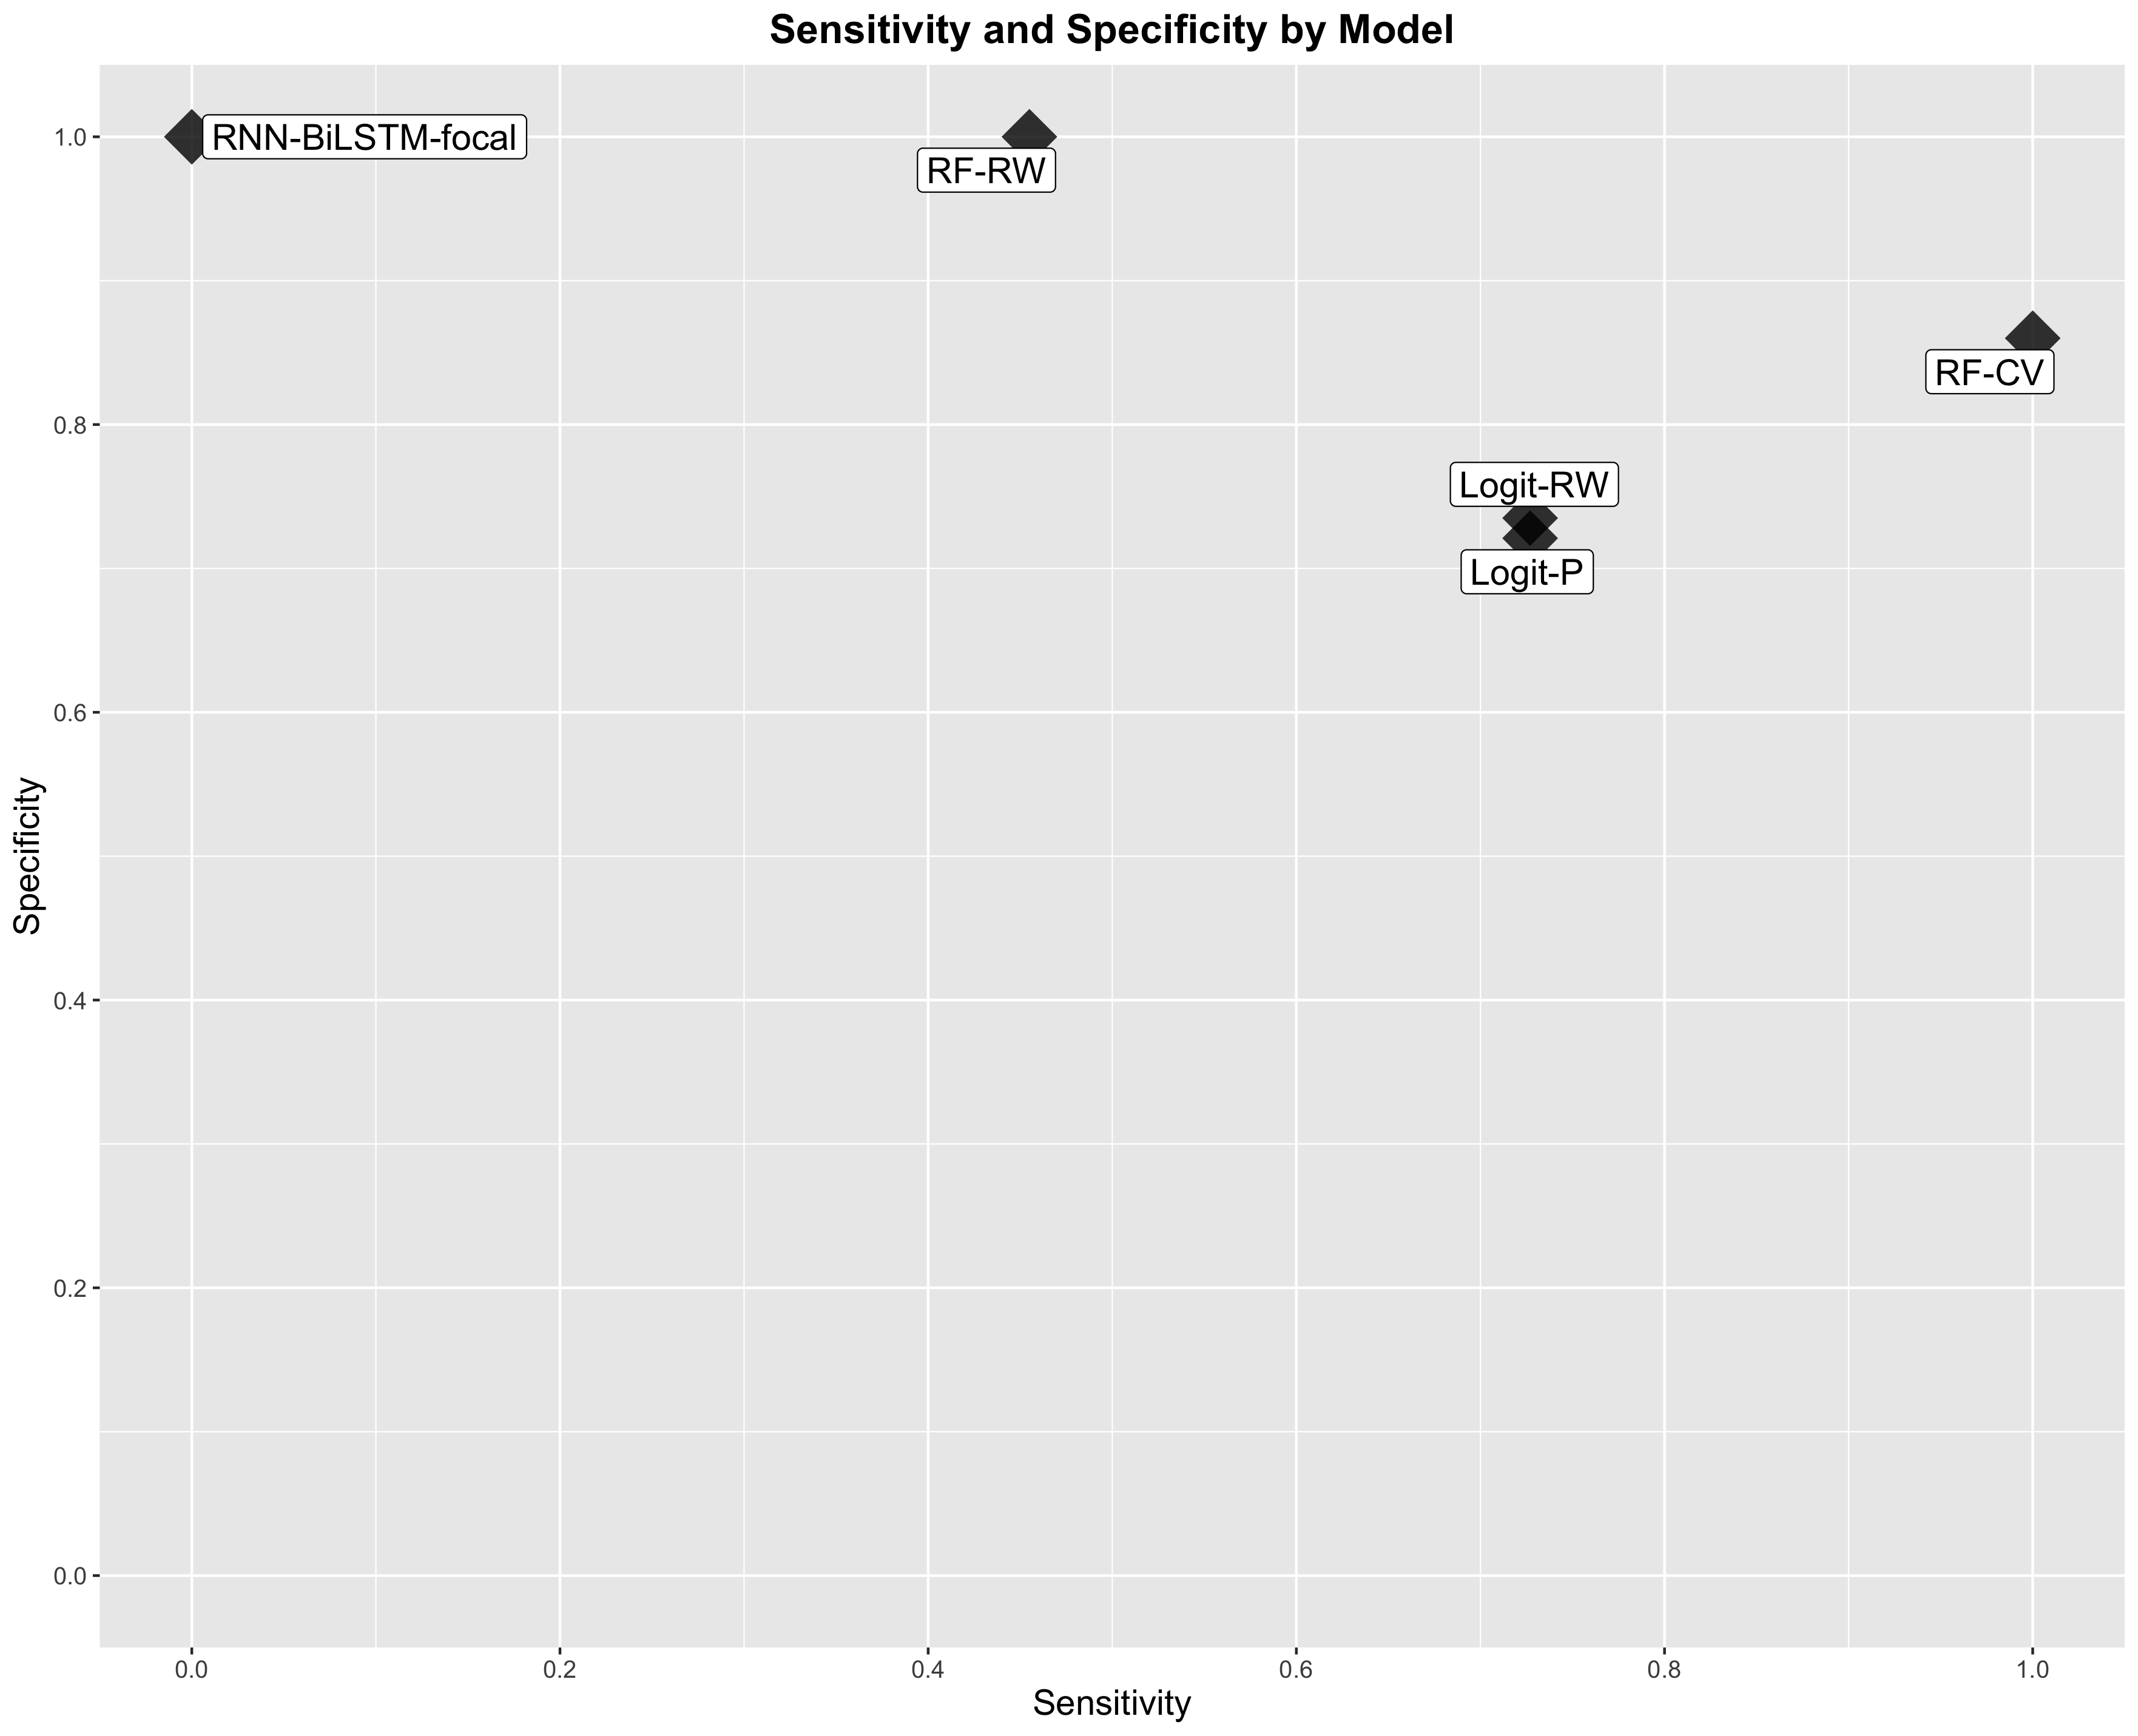
\includegraphics[width=15cm]{res.png}
    \label{fig:res}
\end{figure}

The RF model with a CV-tuned decision threshold performs the best, having a balanced accuracy of 93\%. The sensitivity and specificity show that the model correctly identifies 100\% of the bubble cases and 86\% of the non-bubble cases. Most other models perform decently well, with balanced accuracy rates around 70\%. The RNN model is a disappointment. It performs no better than a naïve model. I will attempt to explain the difference in the predictive power of the models in the discussion section.

Figure~\ref{fig:cv_threshold} and Figure~\ref{fig:rfcv_full} provide more information about the RF-CV model. Figure~\ref{fig:cv_threshold} shows the process of determining the decision threshold. Cross-validation chooses the decision threshold of 0.08 since it yields the lowest balanced error in the CV data. Figure~\ref{fig:rfcv_full} shows the prediction results (red area) of the RF-CV model when imposed on the complete data set. As we can see, the RF-CV model correctly classifies almost all cases. 


\begin{figure}
    \centering
    \caption{The decision threshold tuned by CV}
    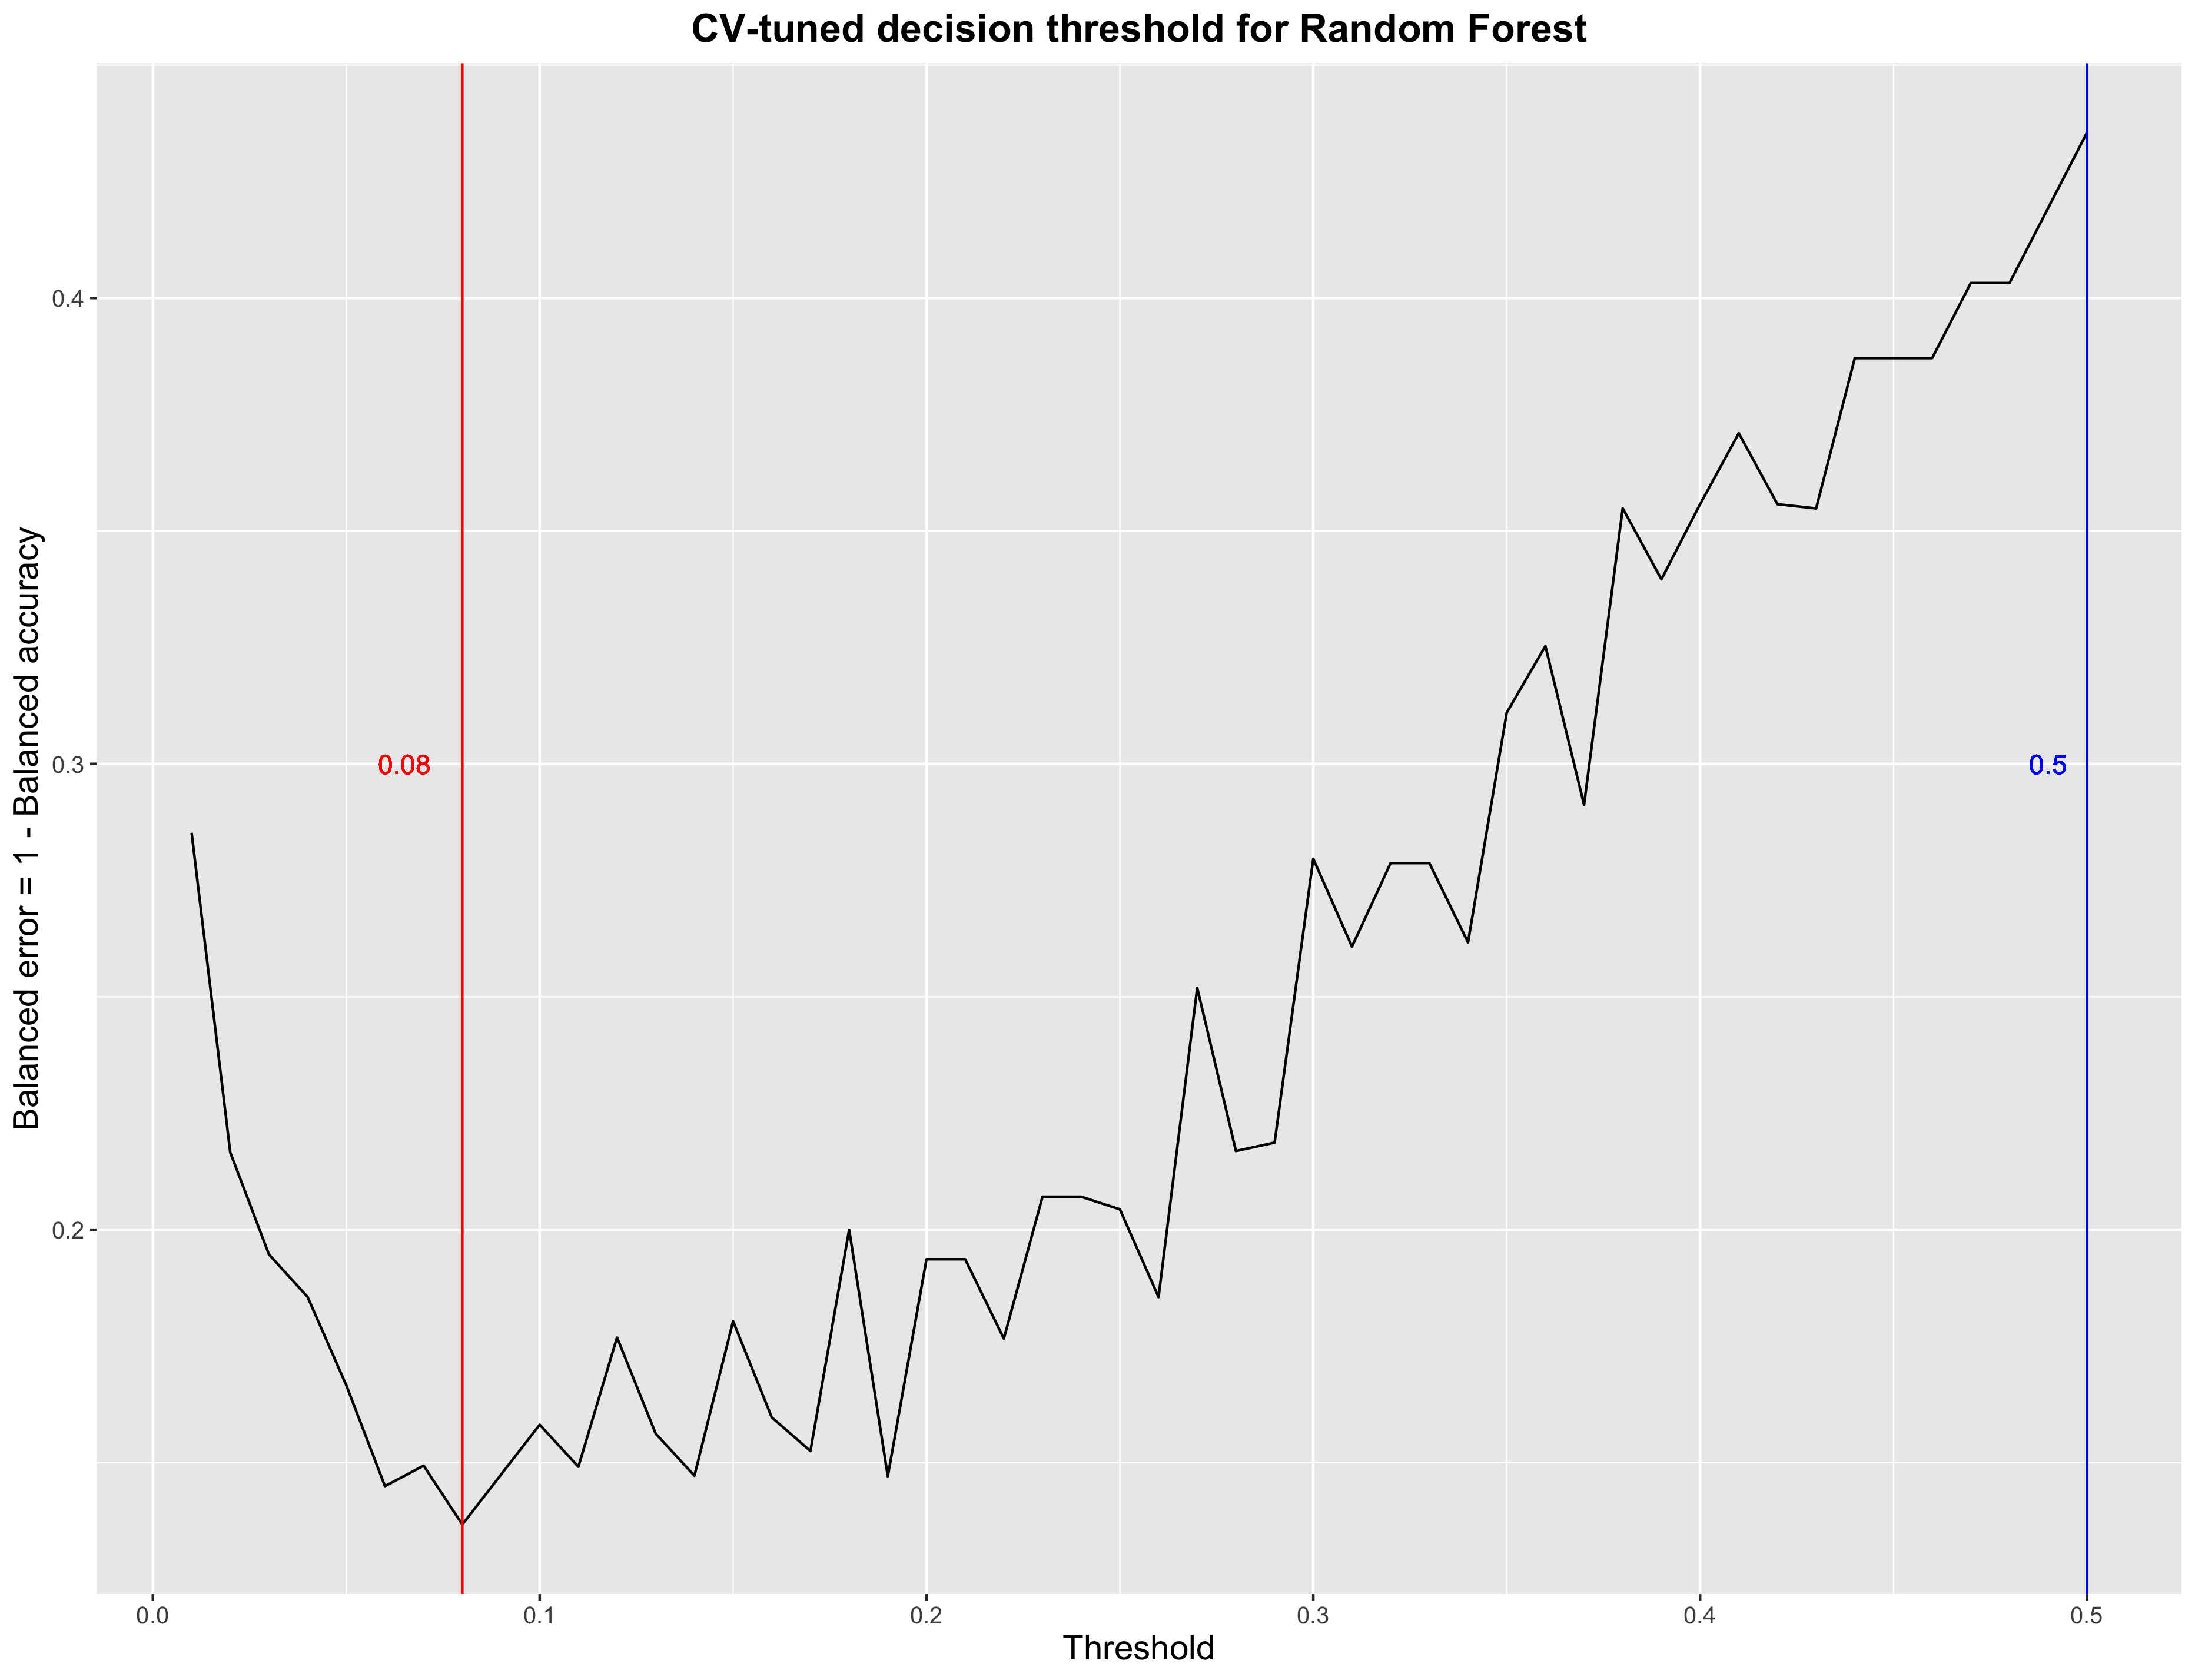
\includegraphics[width=15cm]{cv_threshold.png}
    \label{fig:cv_threshold}
\end{figure}

\begin{figure}
    \centering
    \caption{RF-CV prediction of bubbles}
    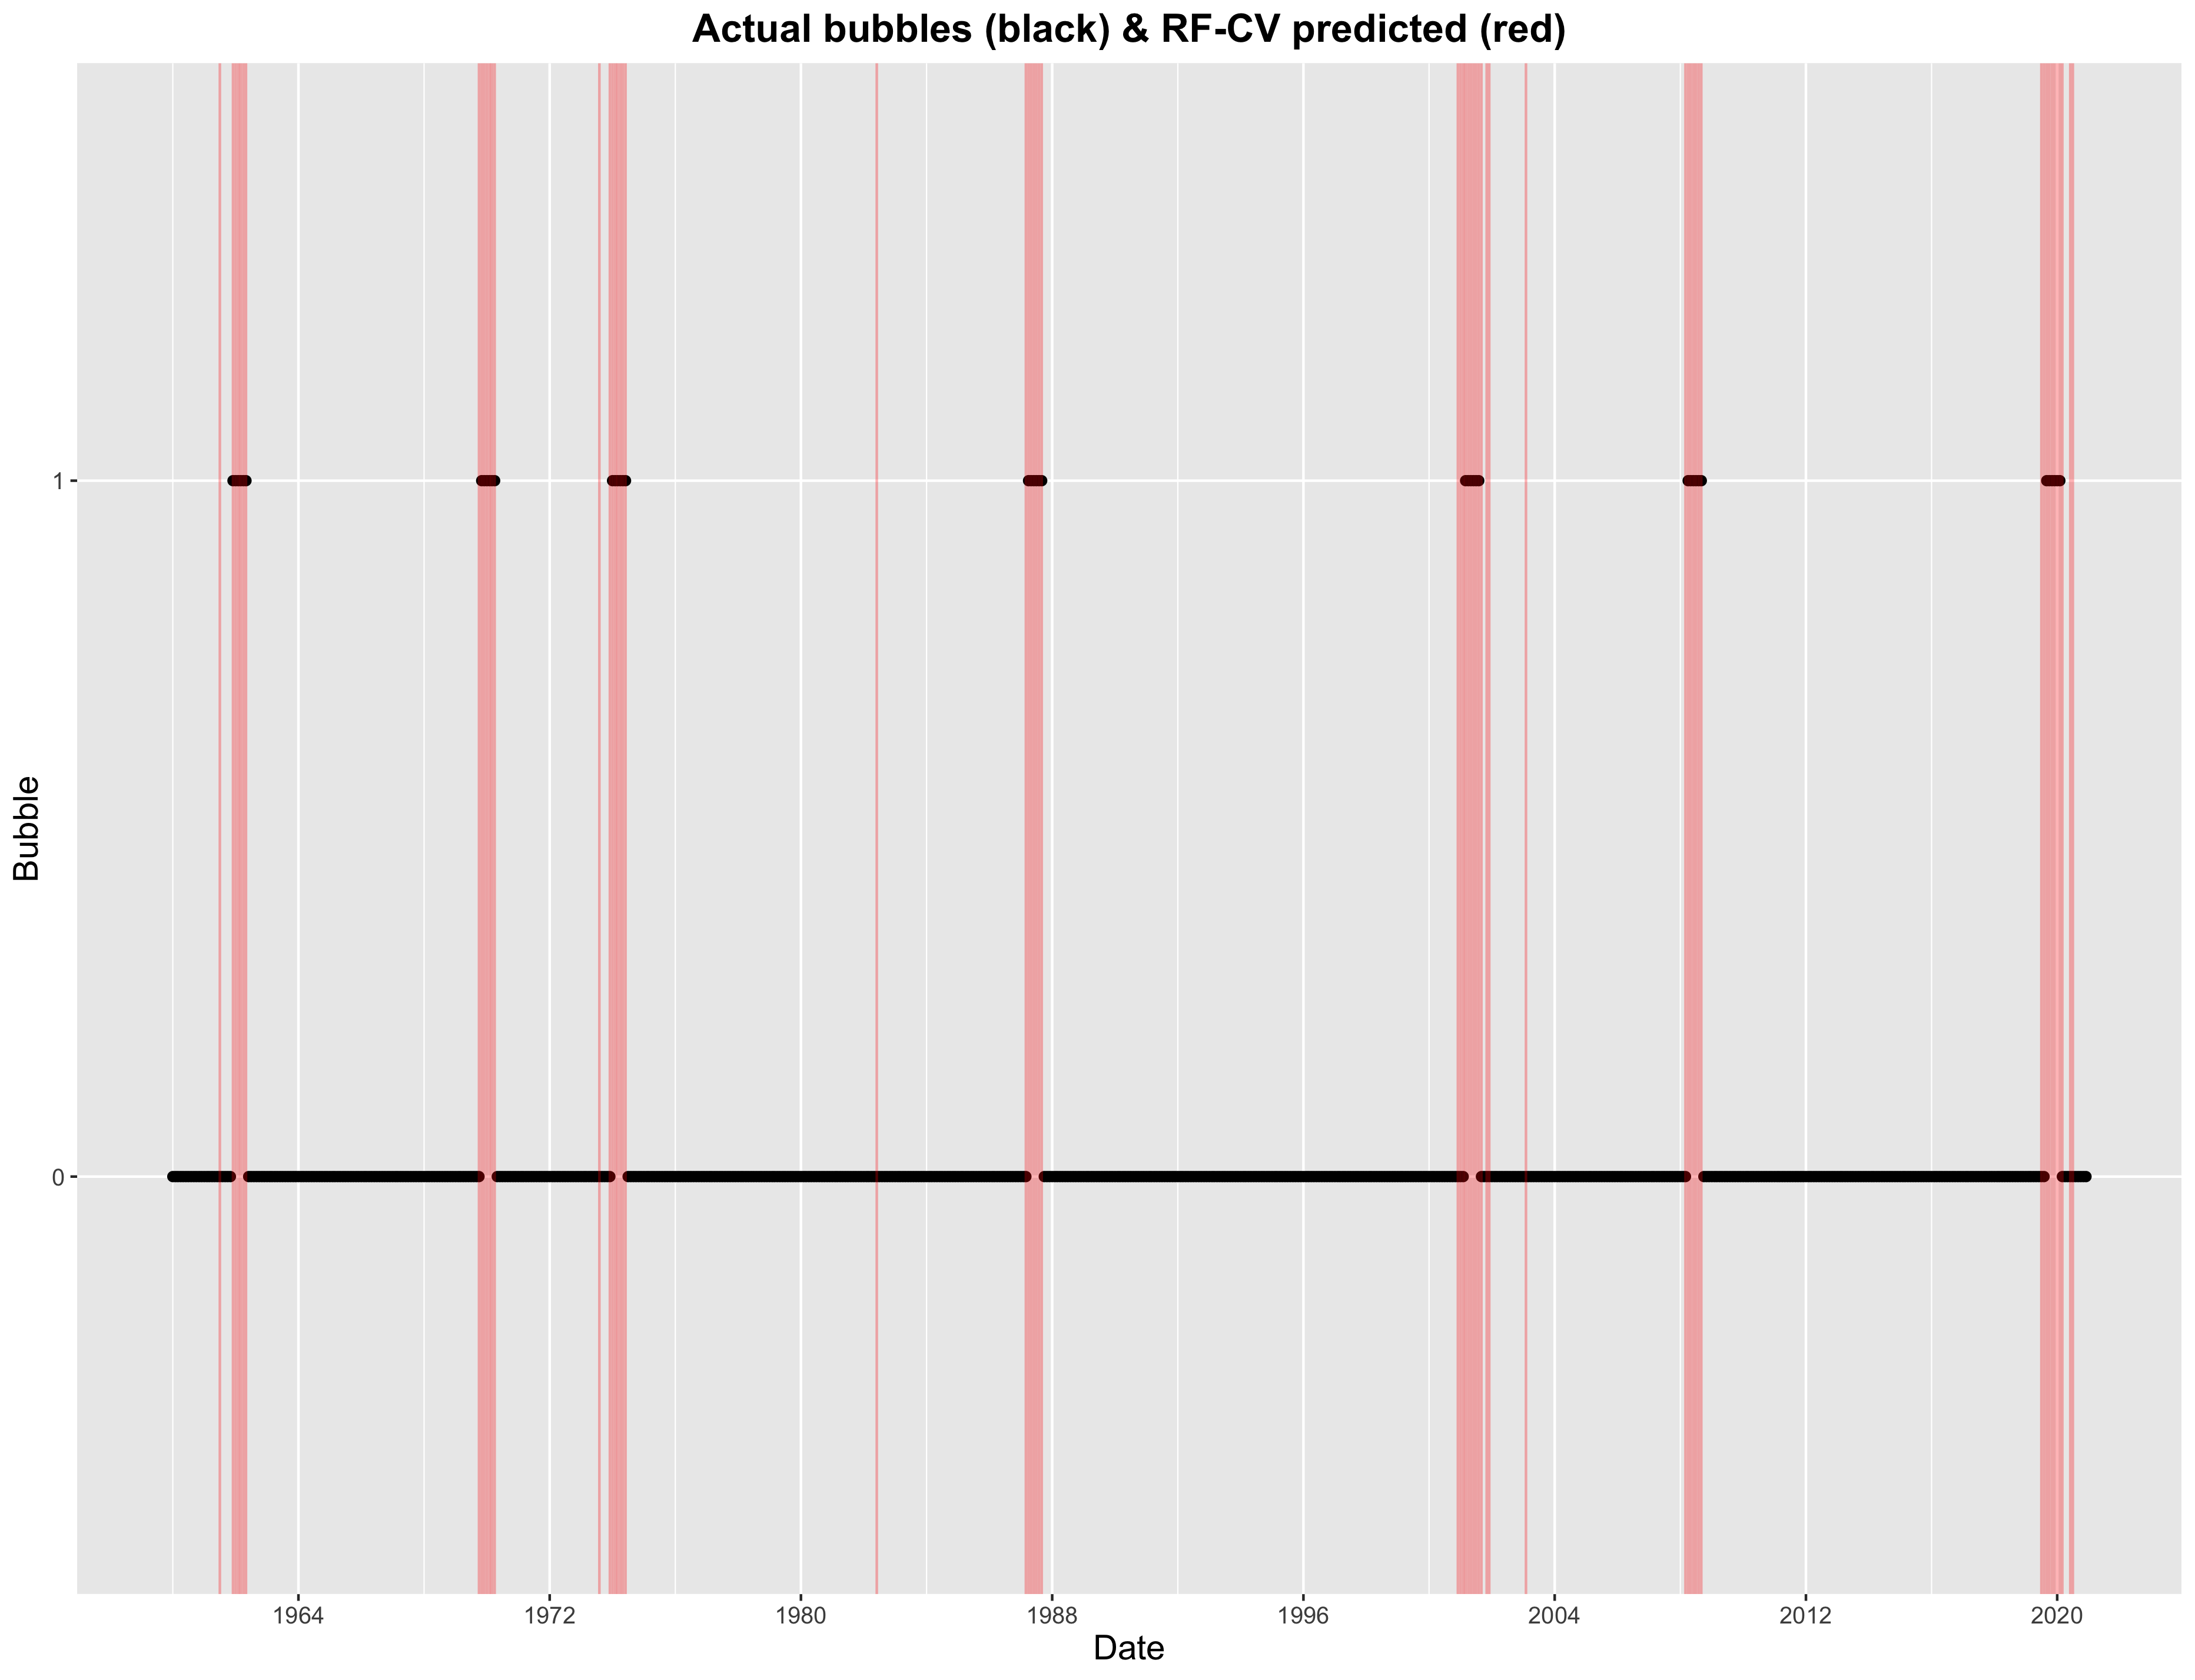
\includegraphics[width=15cm]{rfcv_full.png}
    \label{fig:rfcv_full}
\end{figure}

When feeding with the most recent data (April 2021, the time when this paper is written), the RF-CV model gives the prediction of \emph{bubble}. It suggests that we are likely in a bubble, and financial crashes are likely in the next six months. This result is not financial advice, and I do not recommend the reader to make risky financial decisions based on this result. If the reader still wants to take this result as a reference, I highly recommend the reader to read the discussion section for the limitation of this research before making any decisions.

\subsection{Inference}

There are further insights that we can draw from the research besides the prediction results. We can identify important factors for prediction. I use two of the best performing models for inference: the RF-CV model and the logit-RW model. 

Figure~\ref{fig:varImp} shows the variable importance in the RF-CV model. We see that consumer confidence, long-term investment returns, e.g., 5-year S\&P returns, and fundamental indicators, e.g., market capitalization-to-GDP ratio, are the most important. On the other hand, the short-term S\&P 500 return and short-term macroeconomics data are among the least important features.

\begin{figure}
    \centering
    \caption{The variable importance in the RF-CV model}
    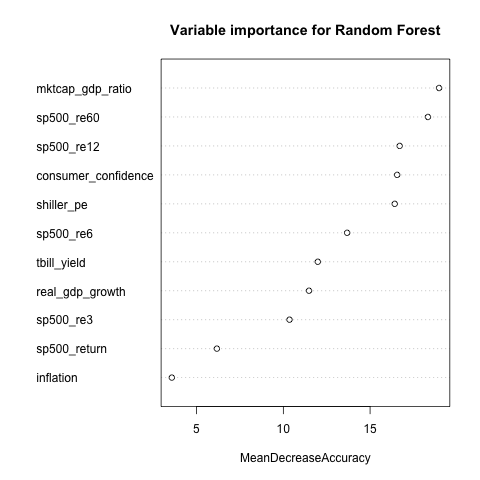
\includegraphics[width=15cm]{varImp.png}
    \label{fig:varImp}
\end{figure}

Table~\ref{tab:logit} shows the regression table for the logit-RW model. It mostly agrees with the results of the RF-CV variable importance plot. The fundamental indicators and long-term investment returns are significant at the 99.9\% confidence level. The 3- and 6- month market returns are not significant. However, contrary to the result of the RF-CV model, the logit-RW model finds inflation and one-month market return significant for prediction.


% Table created by stargazer v.5.2.2 by Marek Hlavac, Harvard University. E-mail: hlavac at fas.harvard.edu
% Date and time: Sun, Apr 18, 2021 - 16:40:33
\begin{table}[!htbp] \centering 
  \caption{} 
  \label{tab:logit} 
\begin{tabular}{@{\extracolsep{5pt}}lc} 
\\[-1.8ex]\hline 
\hline \\[-1.8ex] 
 & \multicolumn{1}{c}{\textit{Dependent variable:}} \\ 
\cline{2-2} 
\\[-1.8ex] & bubble \\ 
\hline \\[-1.8ex] 
 real\_gdp\_growth & 0.012 \\ 
  & (0.034) \\ 
  & \\ 
 inflation & 0.093$^{***}$ \\ 
  & (0.028) \\ 
  & \\ 
 tbill\_yield & 0.234$^{***}$ \\ 
  & (0.071) \\ 
  & \\ 
 shiller\_pe & $-$0.661$^{***}$ \\ 
  & (0.058) \\ 
  & \\ 
 consumer\_confidence & $-$1.279$^{***}$ \\ 
  & (0.154) \\ 
  & \\ 
 mktcap\_gdp\_ratio & 217.538$^{***}$ \\ 
  & (18.556) \\ 
  & \\ 
 sp500\_return & $-$0.092$^{***}$ \\ 
  & (0.033) \\ 
  & \\ 
 sp500\_re3 & 0.034 \\ 
  & (0.022) \\ 
  & \\ 
 sp500\_re6 & $-$0.049$^{**}$ \\ 
  & (0.019) \\ 
  & \\ 
 sp500\_re12 & $-$0.126$^{***}$ \\ 
  & (0.015) \\ 
  & \\ 
 sp500\_re60 & 0.077$^{***}$ \\ 
  & (0.006) \\ 
  & \\ 
 Constant & 115.874$^{***}$ \\ 
  & (14.361) \\ 
  & \\ 
\hline \\[-1.8ex] 
Observations & 1,103 \\ 
Log Likelihood & $-$411.350 \\ 
Akaike Inf. Crit. & 846.699 \\ 
\hline 
\hline \\[-1.8ex] 
\textit{Note:}  & \multicolumn{1}{r}{$^{*}$p$<$0.1; $^{**}$p$<$0.05; $^{***}$p$<$0.01} \\ 
\end{tabular} 
\end{table} 


Based on the above inference, it seems that our model favours the investment philosophy held by value investors, in the context of avoiding market crashes. If the stock prices are too high for corporate earnings and national production, it would be wise to heed the risks of market crashes. Also, these inference results explain why the machine learning models from previous studies do not perform well. As mentioned in the background section, most of the previous machine learning studies for predicting financial crashes only include short-term market return data as features. Those variables have the lowest predictive power among all the input variables I select.


    \section{Discussion}

\subsection{Model diagnosis}

Having seen the model performance in Table~\ref{tab:res}, it is natural to ask why certain models perform better than others. While it is not surprising that the logistic regression models perform less well than more complex models, it is worthwhile to explore why the RF-RW model and the RNN-BiLSTM-focal model do not perform as well as the RF-CV model.

\subsubsection{RF-RW}

After an investigation of the model performance on the training data, I find that there is an overfitting problem for the RF-RW model. The model performs worse on the testing data than on the training data. As shown in Table~\ref{tab:overfit}, the RF-RW model has a 99.3\% balanced accuracy rate on the training data but only 72.7\% on the testing data. This implies that the model fits too much on the patterns in the training data. On the other hand, the RF-CV model does not have this problem.

\begin{table}
    \centering
    \begin{tabular}{lllll}
    \cline{1-3}
    \multicolumn{1}{|l|}{}      & \multicolumn{1}{l|}{Training Data} & \multicolumn{1}{l|}{Testing Data} &  &  \\ \cline{1-3}
    \multicolumn{1}{|l|}{RF-CV} & \multicolumn{1}{l|}{89.5\%}         & \multicolumn{1}{l|}{93.0\%}        &  &  \\ \cline{1-3}
    \multicolumn{1}{|l|}{RF-RW} & \multicolumn{1}{l|}{99.3\%}         & \multicolumn{1}{l|}{72.7\%}        &  &  \\ \cline{1-3}
                                &                                    &                                   &  & 
    \end{tabular}
    \caption{The Balanced Accuracy of RF-RW and RF-CV on the training data and the testing data}
    \label{tab:overfit}
\end{table}

Why would the RF-RW overfit but not the RF-CV? It might be that the re-weighting method makes the model over-trained for the bubble cases in the training data. The re-weighting method replicates the bubble cases, which could cause the model to fit too much on peculiar bubble patterns in the training data. The patterns are not universal for all bubble cases, and they are likely not to be presented in the testing data. This is perhaps why the RF-RW model performs worse on the testing data. On the other hand, the RF-CV alters the decision threshold. This method makes the model focuses on the bubble cases generally, but not restricted to cases seen in the training data. Without the over-training on the peculiar bubble patterns in the training data, the RF-CV model avoids the overfitting problem.

\subsubsection{RNN-BiLSTM-focal}

For the RNN-BiLSTM-focal model, its prediction results are no better than that of a naïve predictor. This is quite a disappointment given the relevant research that endorses the model. It is natural to suspect that the poor result is due to a particular model configuration, and a calibration of the model can improve the performance. Following this line of reasoning, I have tried various techniques, including,

\begin{enumerate}
    \item Adjusting hyperparameters: the number of neurons, the number of layers, the learning rate, the batch size
    \item Changing the type of layers: BiLSTM, LSTM, dense layers
    \item Changing the loss function: adjusting the parameters of the focal loss function
    \item Re-assigning the training and testing data: measure the model performance on a new randomly-selected testing data
    \item Combinations of the above
\end{enumerate}

However, none of these techniques works. The performance of the model does not see any significant improvement. While the above techniques cannot fully dismiss the suspicion of insufficient model calibration, it shows that at least simple model re-configuration does not help.

I examined the probability output of the model to analyze the problem. The distribution of the probability output is shown in Figure~\ref{fig:rnn}. It shows that the variance of probability outputs of the model is small: almost all outputs are clustered around 0.37. Also, the outputs of bubbles and non-bubbles overlap with each other. The model cannot distinguish the two based on the output. Based on this probability output, I suspect that the model is under-trained. It is likely because the model is too complex for our data size. A study on the impacts of data size on LSTM efficiency finds that three-year daily data is required for training an effective model \parencite{datasize}. Three-year daily data is approximately 1000 data points. In this study, we only have 556 data points to train the RNN. It could be that the training data is insufficient to train the RNN model. 

\begin{figure}
    \centering
    \caption{The probability output of RNN-BiLSTM-focal}
    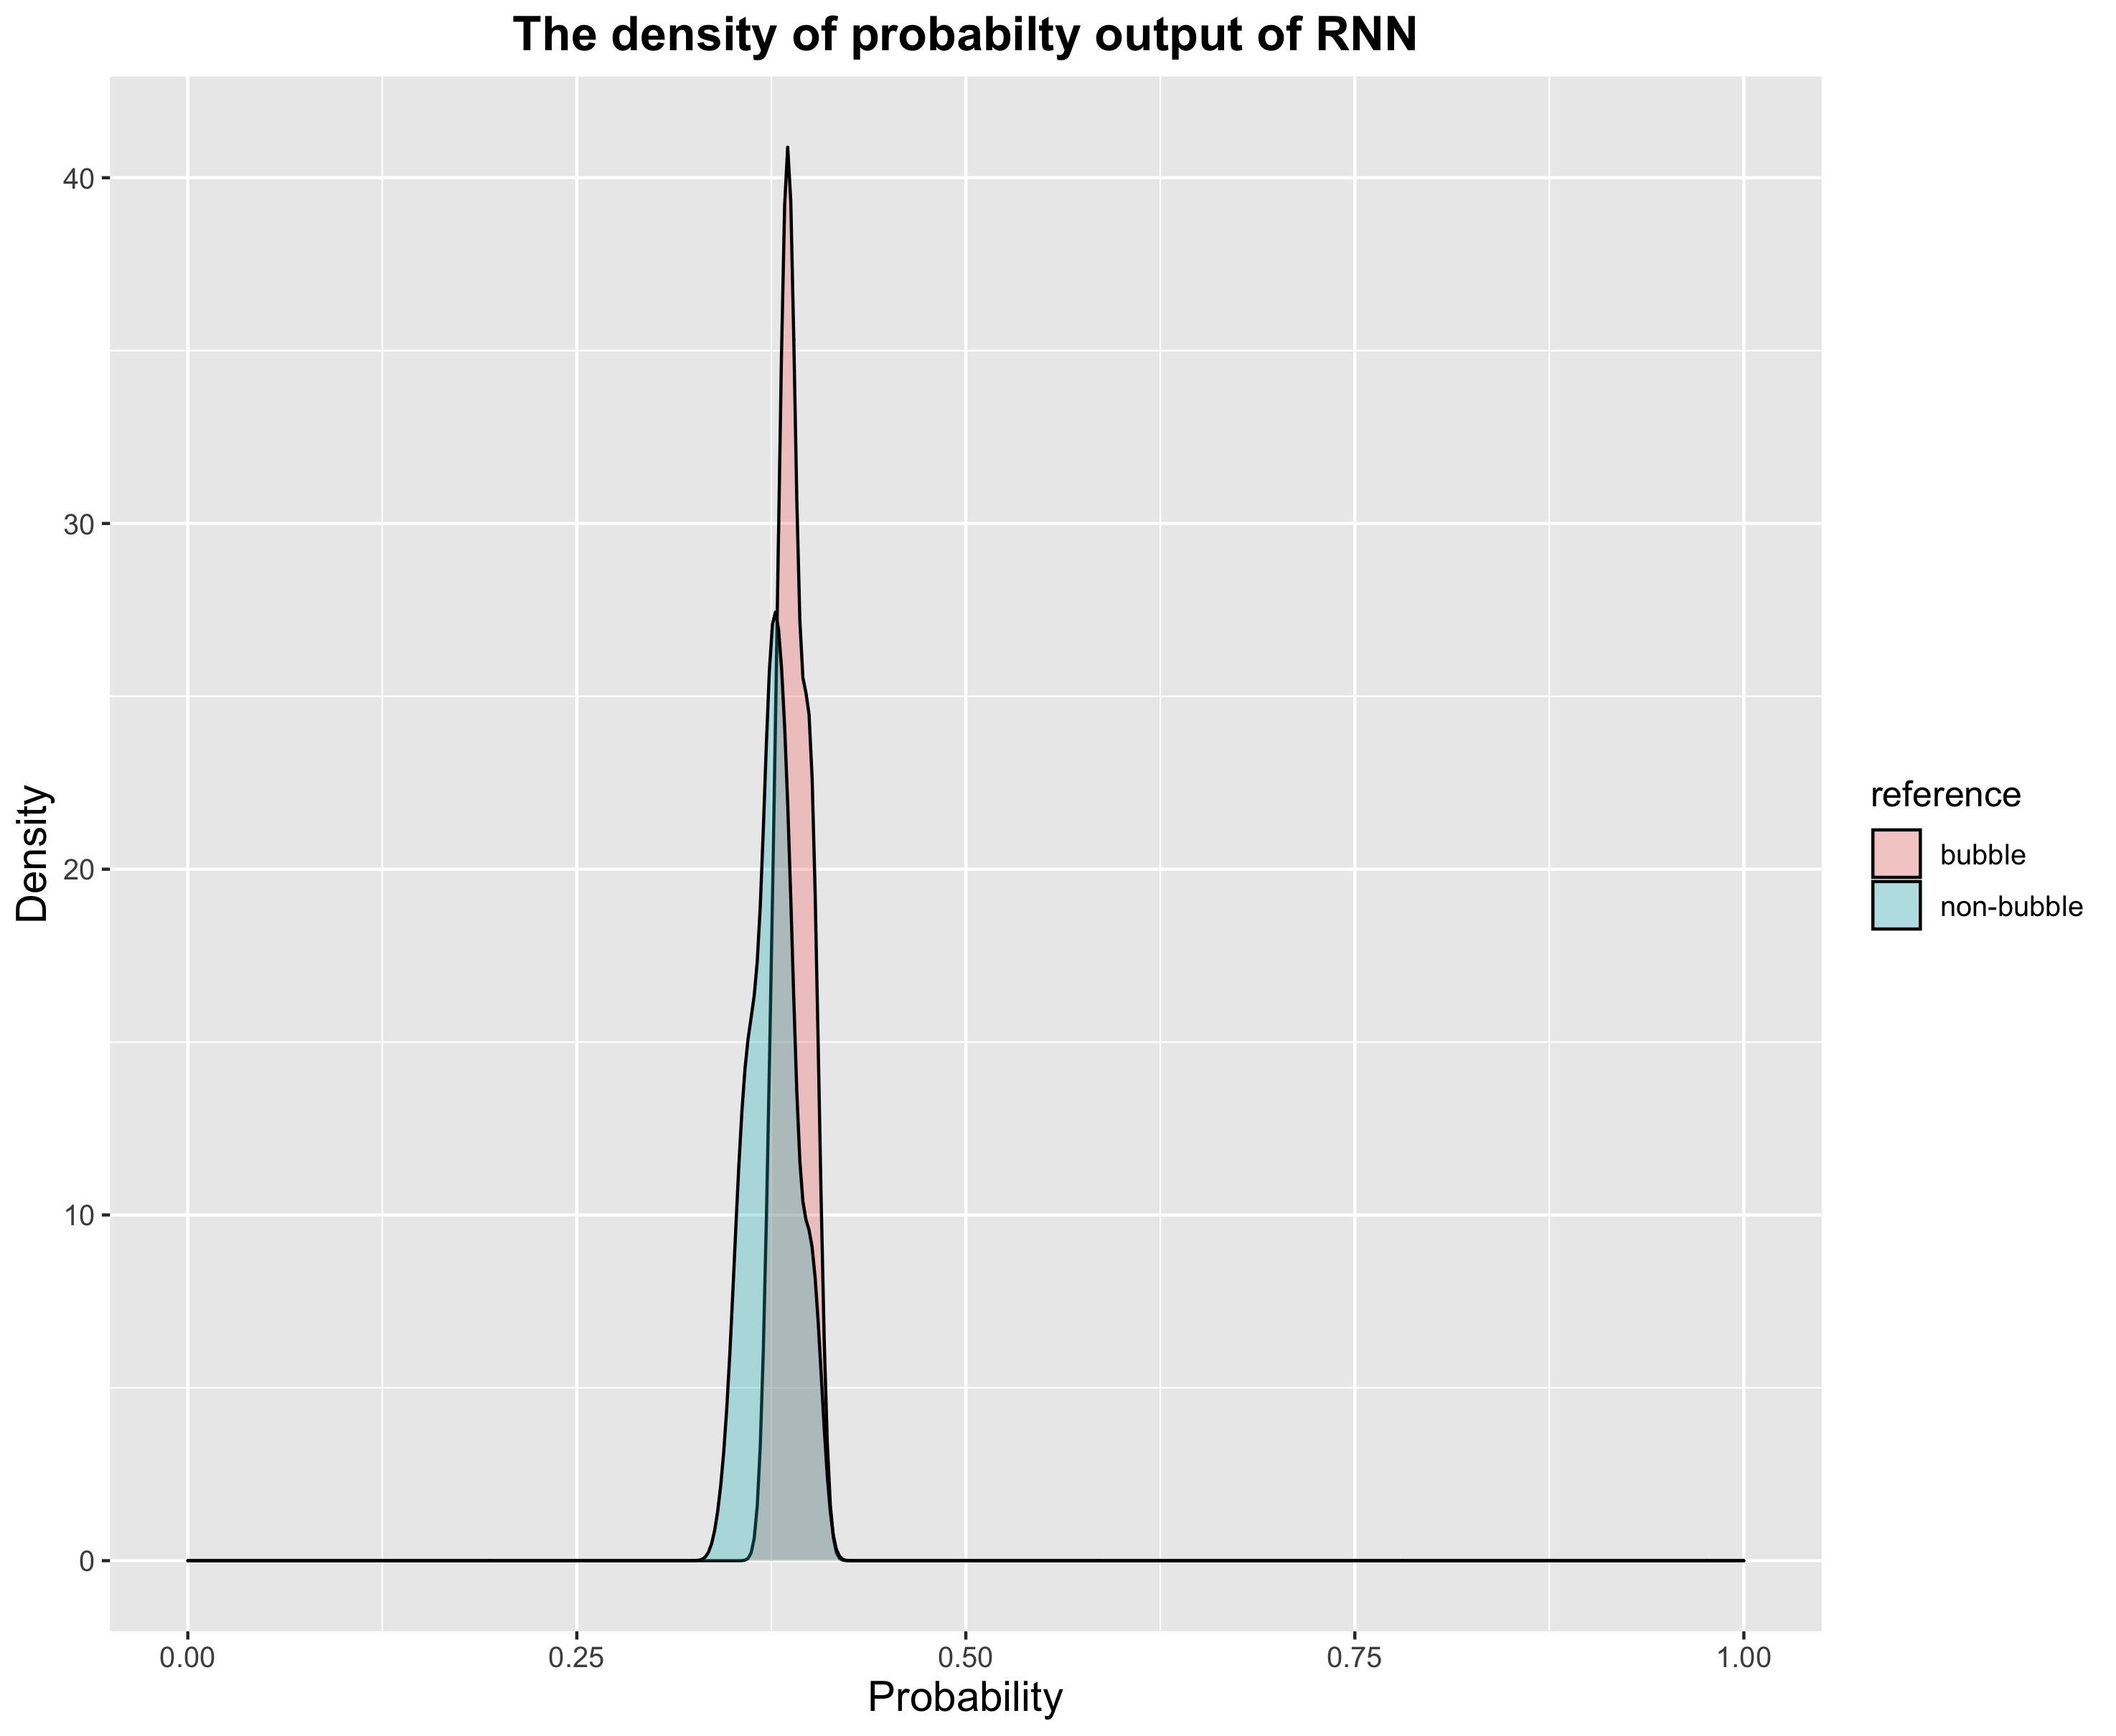
\includegraphics[width=15cm]{rnn.png}
    \label{fig:rnn}
\end{figure}


It is worth noting that the above model diagnoses for the RF-RW model and the RNN-BiLSTM-focal model are largely speculative. Due to the complexities of the models, there does not seem to be an easy way to check my explanations.

\subsection{Robustness analysis}

I did the robustness analysis for the best performing model, the RF-CV model. As discussed in the data section, the quantitative definitions of market crashes and bubbles are rather arbitrary. To check the model performance under different definitions, I alter the “one percentile” and “six months” part of my definition. The results are shown in Table~\ref{tab:rob}.

% latex table generated in R 4.0.3 by xtable 1.8-4 package
% Sun Apr 18 19:24:41 2021
\begin{table}[ht]
\centering
\begin{tabular}{rrrrr}
  \hline
 & 0.005 & 0.01 & 0.015 & 0.05 \\ 
  \hline
3 & 0.67 & 0.68 & 0.72 & 0.80 \\ 
  5 & 0.91 & 0.99 & 0.86 & 0.85 \\ 
  6 & 0.99 & 0.94 & 0.86 & 0.90 \\ 
  7 & 0.97 & 0.96 & 0.88 & 0.90 \\ 
  12 & 0.97 & 0.93 & 0.91 & 0.88 \\ 
   \hline
\end{tabular}
\caption{Balanced accuracy of RF-CV with different quantiles (column) and periods (row)} 
\label{tab:rob}
\end{table}


We see the model performance is reasonably robust. The model has balance accuracy rates around 95\% if the percentile in the market crash definition is lower than 1 and the number of periods in the bubble definition is between 5 and 12. However, the model performs worse for a short-term bubble definition (3-month period) and a less extreme definition of market crashes (5 percentile). This suggests that our model is limited in predicting extreme market crashes in a relatively long time frame. 

The result is not unexpected. The most important factors of the model are market fundamental indicators and long-term trends, so it is plausible that the model based on these factors has less predictive power in the short term. Besides, the method of changing the decision threshold is deployed specifically for the imbalanced data problem. If the data is less imbalanced due to a less extreme market crash definition, this method will not be effective.

\subsection{Limitations}

Besides the limitation that the model is unsuitable for short-term and less extreme market crashes prediction, as discussed in the robustness analysis subsection, two other limitations are worth mentioning.

The first limitation is regarding the interpretation of the results. A balanced accuracy rate should not be confused with a precision rate. A balanced accuracy rate stands for the balanced percentage of correctly identified cases. On the other hand, a precision rate means among all cases that are predicted as bubbles, the percentage of cases that are actual bubbles. While the RF-CV model has a high balanced accuracy rate, the precision rate is much lower, at 36.7\%. This means that if the model gives a \emph{bubble} prediction, there is only a 36.7\% possibility that a market crash would take place in the next six months. From a practical perspective, the user of the model should heed the possibility of false alarms when the model predicts bubbles.

Why would the two metrics differ? It can be best illustrated by the confusion matrix of the model prediction. As shown in Table~\ref{tab:cfm}, the model correctly identifies most of the cases in both categories, but precision (11/30) is still modest. Although the proportion of misclassified non-bubble cases is low (19/177), the number is non-negligible. Non-bubble cases are much more than bubble cases so that a small portion of misclassified non-bubbles (19) is more than the correctly identified bubbles (11). This drives the precision much lower than the accuracy. 

% latex table generated in R 4.0.3 by xtable 1.8-4 package
% Mon Apr 19 01:56:36 2021
\begin{table}[ht]
\centering
\begin{tabular}{rrr}
  \hline
 & bubble & non-bubble \\ 
  \hline
bubble &  11 &  19 \\ 
  non-bubble &   0 & 117 \\ 
   \hline
\end{tabular}
\caption{Confusion matrix of the RF-CV model, reference(columns) and prediction(rows)} 
\label{tab:cfm}
\end{table}


The second limitation is that the training data and testing data are not independent. While they are split randomly from the full data, they are both from a similar period. For example, the data of May 2008 is in the training set, whereas the data of June 2008 could be in the testing set. The two periods are positively correlated due to their proximity in time. At the training stage, the model fitter learns that May 2008 is in a situation of bubble and incorporates its pattern into the model. When faced with the data of June 2008 in the testing set, it is easy for the model to correctly classify it as a bubble case since it has seen a similar instance in the training data. However, for real-world applications, the model would encounter cases that have much less similarity to the training data. When asked to check if there is a bubble as of April 2021, the model does not have any information about whether March 2021 or May 2021 has a bubble or not. This is a harder problem for the model than the question of June 2008. It is dubious if the model would perform equally well. In short, the dependence between the training data and the testing data is likely to make the testing performance of the models overstated.


    \section{Conclusion}

I start this research with the purpose to detect equity bubbles and predict financial crashes. I find that previous empirical studies are limited by their theoretical assumptions or feature selection techniques. To overcome these limitations, I choose the model-free machine learning approach, and the features are selected based on theories but do not rely on theories. Based on the nature of the research problem and relevant studies, I use logistic regression, Random Forests, and Recurrent Neural Networks as my models. To tackle the challenge of the imbalanced output variable, I change the decision thresholds, re-sample the data for weighting, and adopt an asymmetric loss function.

The key findings of the research are as follows. The primary research goal is realized — I find a high-performance predictor. The Random Forest with CV-tuned performs the best, with a balanced accuracy rate of 93.0\%. The high performance of the model shows that machine learning is a viable method for equity bubble detection. In particular, it confirms the findings of \textcite{LinSurvey} that ensemble learning methods are promising in the field of financial crisis prediction. Also, the unsatisfactory result of the RNN model suggests that deep learning methods may not always outperform traditional methods. Especially in the case of small and medium data size, the complexity of the RNN model could lead to under-training. In the research, I also identified important factors for the prediction. Behind the predictive models, it is found that long-term market returns and market fundamental indicators have the highest predictive power, whereas short-term market returns and macroeconomic data are not as important. Finally, it is worth mentioning that the best-performing model predicts that market crashes are likely in the next few months (starting from April 2021).

The research has two main contributions. First, I use a new research methodology. I improve the prediction accuracy of machine learning methods by utilizing variable importance insights from economics theories. The result of this research encourages future machine learning studies to select more features based on theories. Second, I build a high-performing predictor (RF-CV) for detecting equity bubbles and predicting market crashes. While the caveat is that the model only has a modest precision rate, I believe the model can be useful for investment practitioners. For example, policymakers can use it as an early warning system, and investors can use it as a risk management tool.

The research is limited by the prediction horizon and the type of market downturn. The model cannot be generalized to short-term, e.g., 1-month prediction, and mild market crash prediction. From a practical perspective, the model does not have a high precision rate so that it is prone to send false alarms. Besides, it is suspected that a positive correlation between the training data and the testing data makes the model overstate its testing performance. 

Future research is needed to analyze deeper and overcome the correlation problem. Also, the extension of this research can include more features into the predictive models. Lag values can be included to better capture the time-series pattern of the data. Besides, through feature engineering, we can use the result of econometric tests as input variables. For example, for the test proposed by \textcite{craine1993}, we can include a dummy variable of whether the non-stationary null hypothesis is rejected. Using the same methodology as this research, feature engineering is not subjected to the theoretical challenge such as the joint hypothesis problem since it only includes the test result as a feature. In this way, we can not only include potentially important factors but also test the empirical performance of the econometric tests. Future research can also consider including more machine learning algorithms such as gradient boosting and support vector machines. Hopefully, using these methods, future research can improve on the findings of this research and make the results more robust.

    \clearpage
    \printbibliography
\end{document}